The primary interface to the PFA is through a number of memory-mapped queues:
\gls{freeq}, \gls{newq}, and \gls{evictq}. The \gls{freeq} contains unused page frames that the PFA can
use for fetching new pages, the \gls{newq} reports any recently fetched pages to the
OS bookkeeping thread, and the \gls{evictq} contains a list of local pages that
should be stored in remote memory. Using these queues, execution proceeds as
follows:

\paragraph{Eviction}
The PFA handles all communication with the memory blade. This includes page
eviction. The basic procedure is as follows (see figure \ref{fig:evict_detail}
for a detailed description):

\begin{outline}[enumerate]
    \1 The OS identifies pages that should be stored remotely.
    \1 It evicts them explicitly by writing to the \gls{evictq}.
    \1 The OS stores a page identifier in the PTE and marks it as remote.
\end{outline}

\begin{figure}[h] \centering
  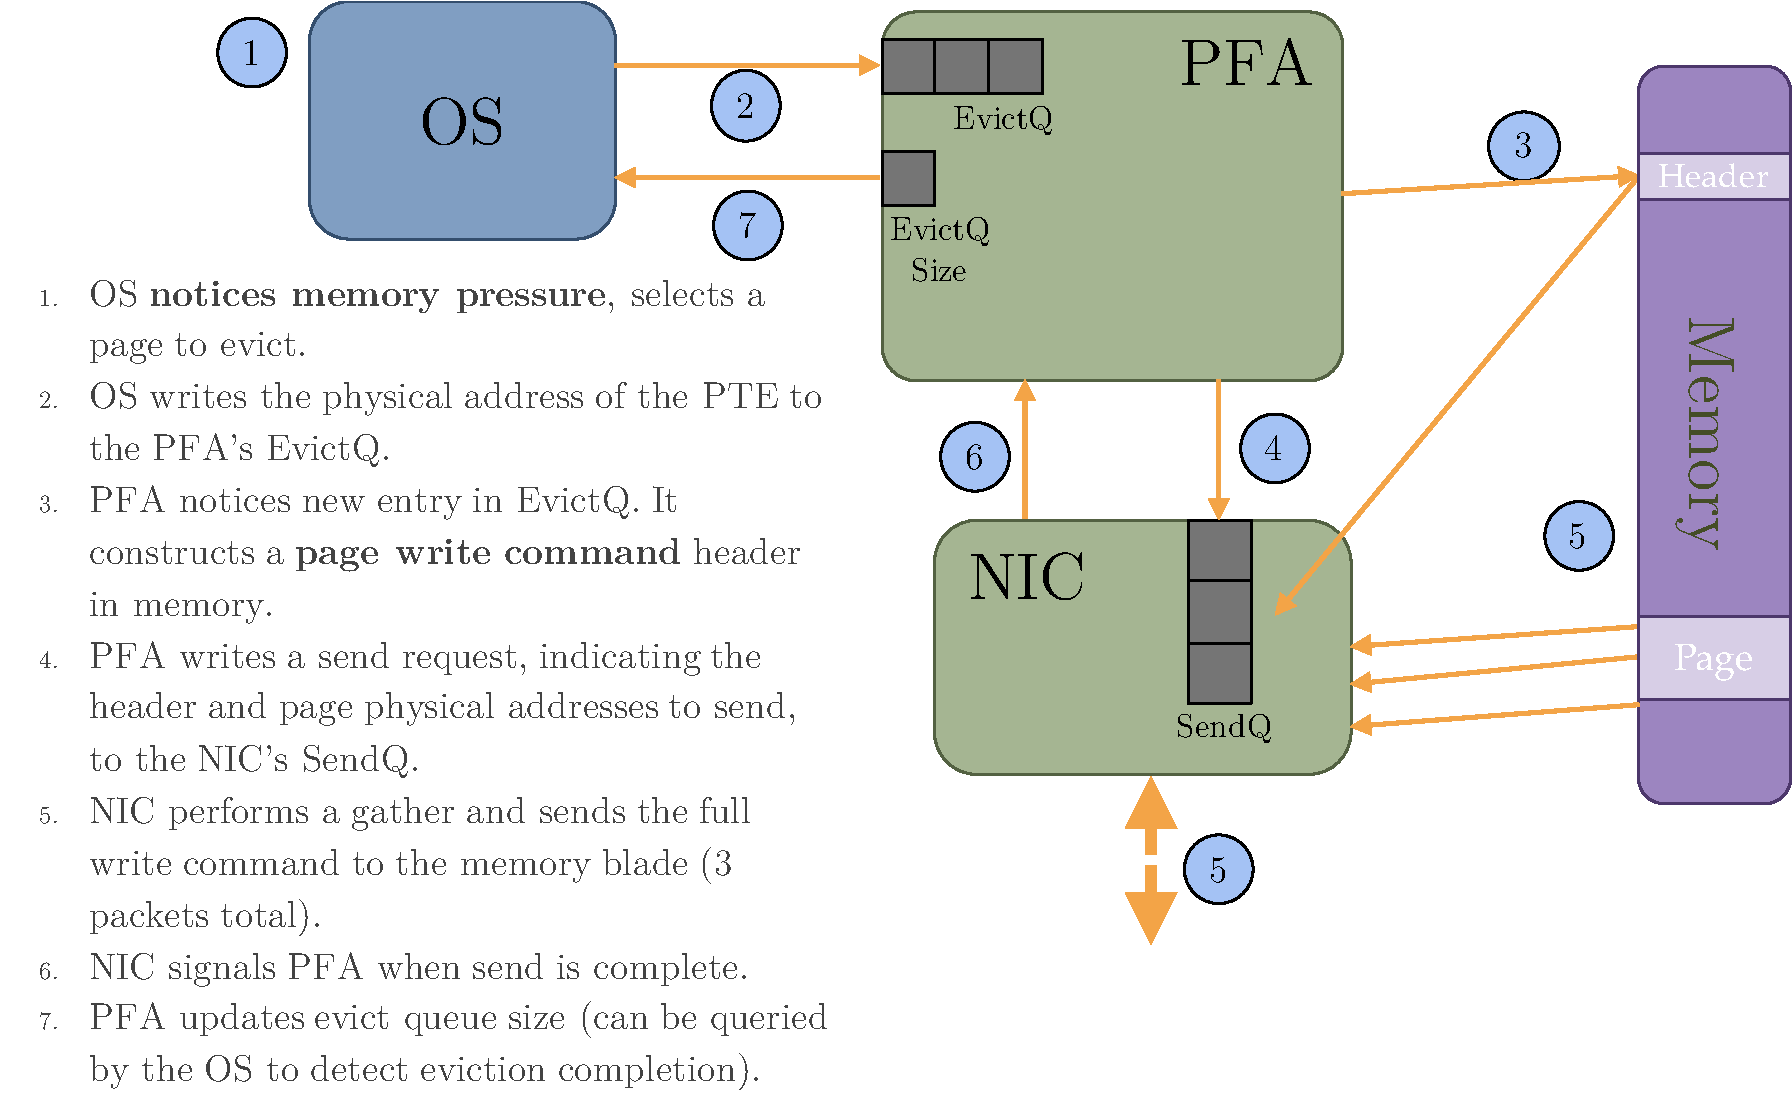
\includegraphics[width=\columnwidth]{figs/pfa_evict_detail.pdf}
  \vspace{-5mm}
  \caption{Detailed eviction flow}
  \label{fig:evict_detail}
\end{figure}

In addition to the three main queues, there are a number of other maintenance
registers that are used for querying queue status and initializing the PFA. See
appendix \ref{apx:pfa_spec} for a complete specification. I will mention one status
register here; the EVICT\_STAT register. When a page is placed on the evict
queue, the PFA begins transferring it to remote memory, but does not block
the OS. This allows the OS to perform useful work while the eviction is taking
place, potentially hiding some of the write latency. In order to re-use the
page frame, however, the OS must poll the EVICT\_STAT register to ensure the
write has completed.

\FloatBarrier

\paragraph{Fetch}
The primary function of the PFA is to automatically fetch pages from remote
memory when an application tries to access it. It does this by detecting page
table entries that are marked remote and transparently re-mapping them to the
next available free frame. The basic operation is as follows: 

\begin{outline}[enumerate]
    \1 Application code issues a load/store for the (now remote) page.
    \1 The PFA automatically and synchronously brings the page from remote
       memory and stores it in a free frame.
    \1 The PFA clears the remote bit in the \gls{pte}.
    \1 The PFA pushes the virtual address of the fetched page to the NewQ.
    \1 The application is restarted.
\end{outline}

Figure \ref{fig:fetch_detail} describes the process in more detail.
\begin{figure}[h] \centering
  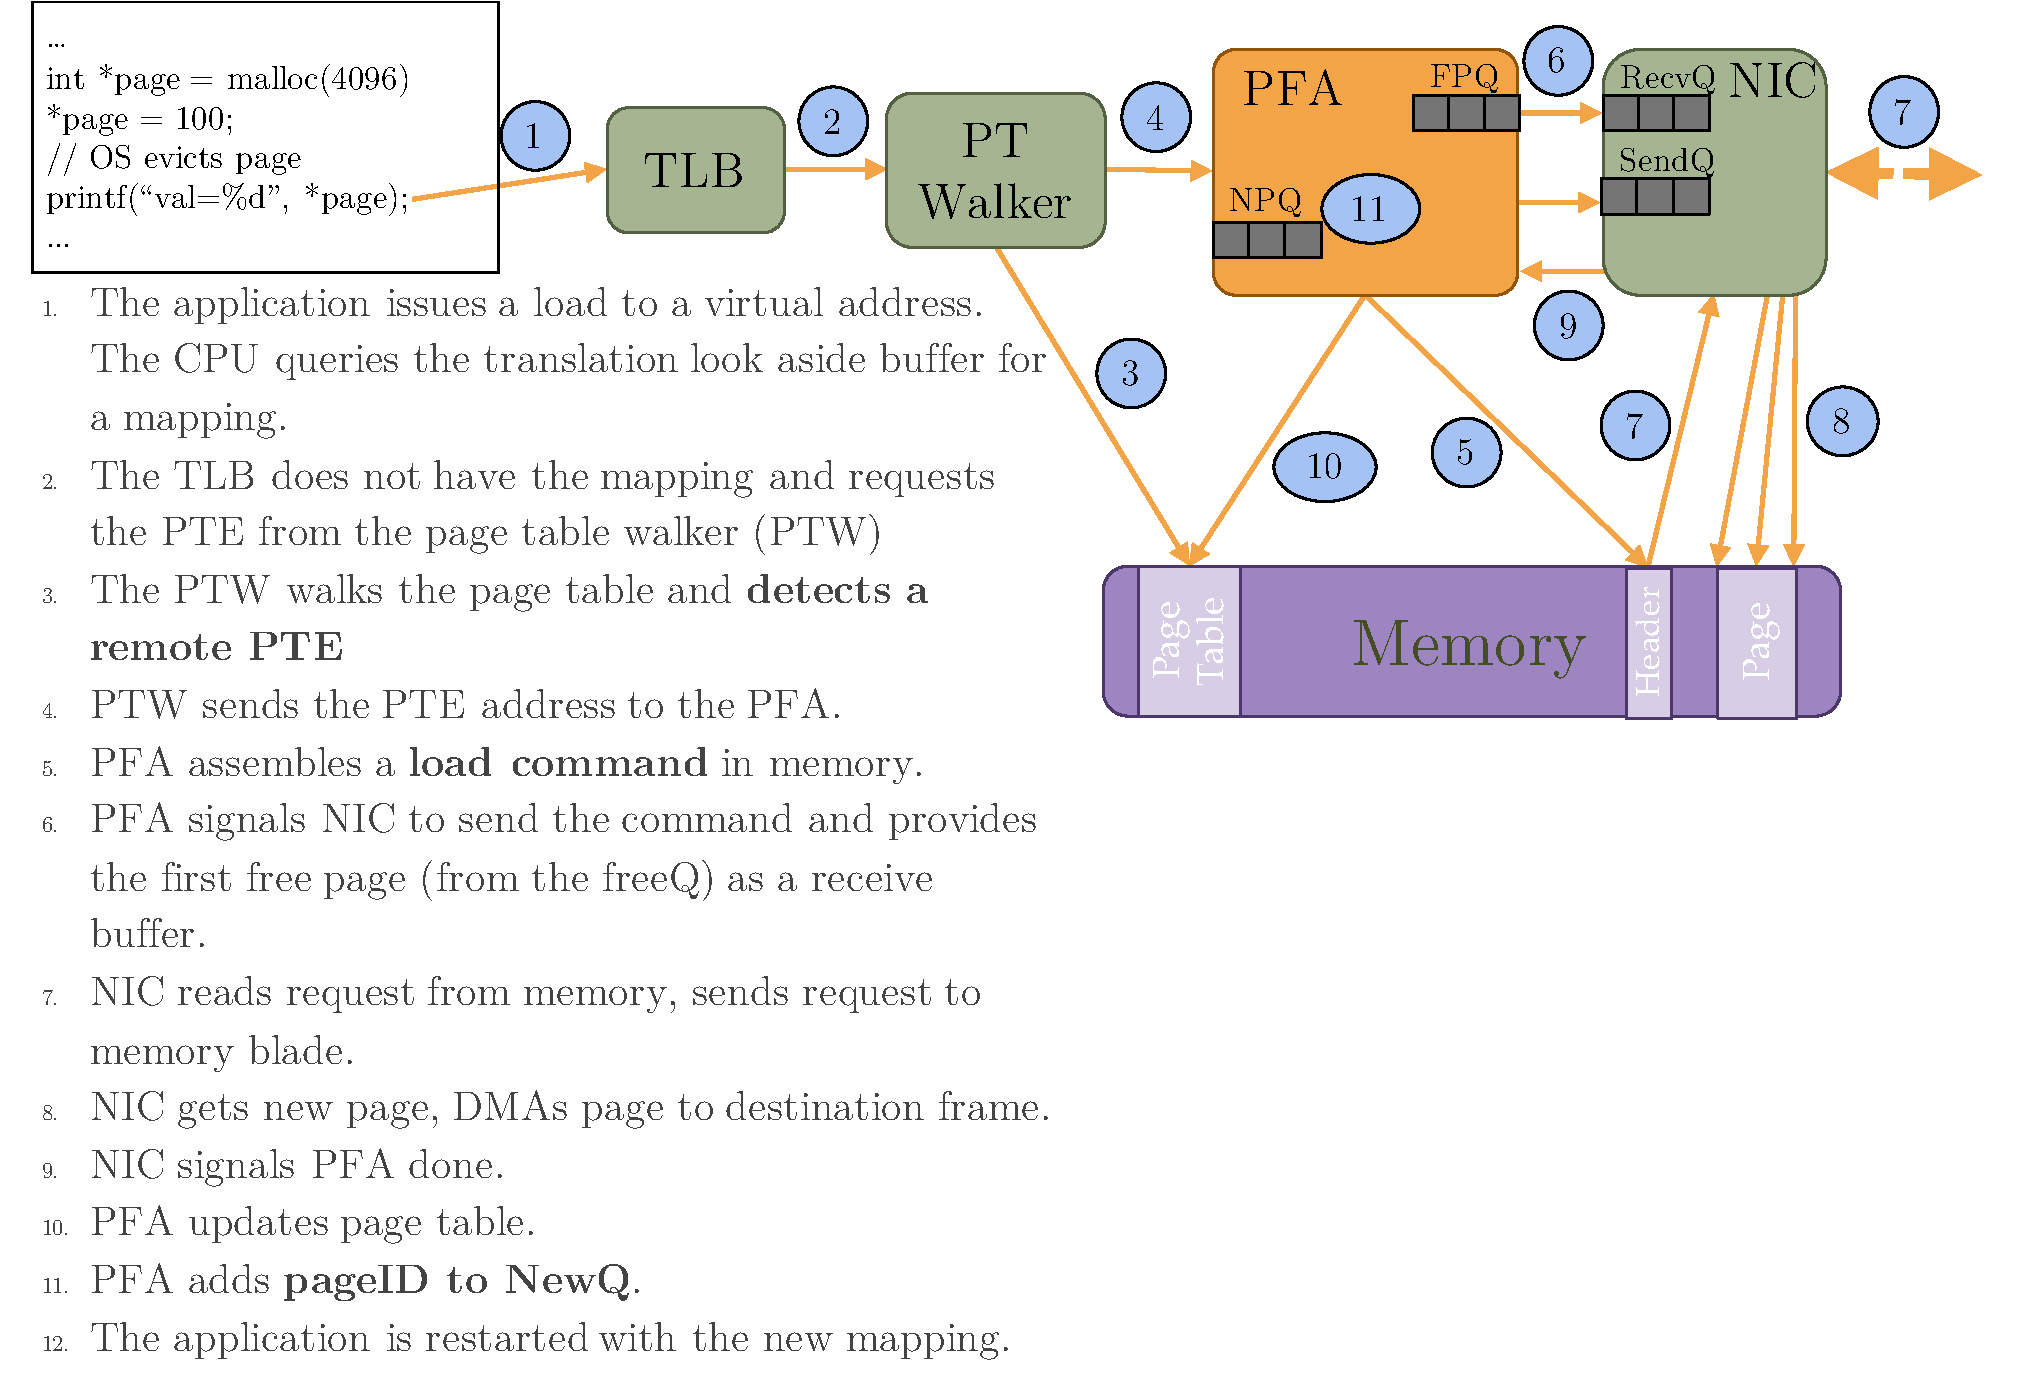
\includegraphics[width=\columnwidth]{figs/pfa_fetch_detail.pdf}
  \vspace{-5mm}
  \caption{Detailed fetch flow}
  \label{fig:fetch_detail}
\end{figure}
\FloatBarrier

\paragraph{Metadata Management}
The OS should ensure that there are sufficient free frames in the \gls{freeq} to
ensure smooth operation. If a remote page is requested and there are no free
frames, the PFA will trap to the OS with a conventional page-fault. The OS must
enqueue one or more free-frames before returning from the interrupt. This may
involve evicting pages synchronously in the page-fault handler.

Similarly, the OS needs to drain the new page queue periodically to ensure it
does not overflow. This will also trap to the OS with a conventional page
fault.

\subsubsection{Page Table Entry} \label{sec:remPTE}
The PFA uses a special PTE format for remote pages (Figure
\ref{fig:pte_format}). The fields are as follows:

\begin{outline}
  \1 \textbf{\gls{pgid}}: This acts as an address in remote memory for the remote
  page. It is used by the PFA to look up pages in remote memory, and for the OS
  to identify each page during bookkeeping.
  \1 \textbf{Prot}: This sets the protection bits that the PFA will use when
  fetching a page. These bits include things like read/write permissions, as
  well as other page metadata (see the RISC-V privileged architecture manual
  for more details \cite{riscv_priv110}).
  \1 \textbf{R}: This bit indicates that a page is remote (when the valid bit
  is clear).
  \1 \textbf{V}: This indicates whether a page is valid.  A valid page is
  currently in main memory and would not trigger a page-fault.  This is also
  referred to as the ``present bit'' in Linux.
\end{outline}

\begin{figure}[h]
  \centering
  \begin{bytefield}[endianness=big,bitwidth=0.016\linewidth]{64}
    \bitheader{0, 1, 2, 12, 40, 63} \\
    \bitbox{24}{Unused} & \bitbox{28}{Page ID} & \bitbox{10}{Prot} &
    \bitbox{1}{\tiny R} & \bitbox{1}{\tiny V} \\
  \end{bytefield}
	\caption{Remote PTE Format. The \textbf{Page ID} is a unique identifier of this page
  and serves as a remote memory address. The \textbf{Prot} field contains the permission
and metadata bits that should be set after a page is fetched (see the RISC-V
specification for details\cite{riscv_priv110}). The \textbf{R} bit indicates
that this page is remote while the \textbf{V} bit indicates that the PTE is not
a valid mapping (needed for backward compatibility).}
	\label{fig:pte_format}
\end{figure}

It is worth noting that the RISC-V instruction set manual specifies that all
bits other than the valid bit are considered ``don't care'' when the valid bit
is clear. This deviation from the standard may be problematic for some OSs, but
is compatible with the Linux kernel. Another interesting feature of this design
is the use of pre-defined protection bits. This includes a valid bit which can
be cleared by the OS before evicting to trigger a page fault on this page
immediately after fetching (a useful debugging feature). Also, bits 8 and 9 
are reserved for software by the RISC-V ISA and can aid the OS in bookkeeping
and debugging (see Section \ref{sec:linuxImpl}).

\subsubsection{Remote Memory Protocol}
When the PFA receives a request for a remote page from the PTW, it must
communicate with a remote \gls{memory blade} to retrieve the appropriate data.
It does this through a custom network protocol. This involves forming network
packets and interfacing with the NIC. For this project we assume an
Ethernet-based network with a \gls{mtu} of \SI{1500}{\byte} and a page size of
\SI{4}{\kilo\byte}, this is not fundamental to the design.  Figures
\ref{fig:write_protocol} and \ref{fig:read_protocol} show the basic operation
of the protocol. See appendix \ref{apx:memblade_spec} for a detailed
description of these packet types. Note that due to the \gls{mtu}, each page
takes 3 packets to transfer.
\begin{figure}[h]
    \centering
    \begin{sequencediagram}
        \newinst{c}{PFA}
        \newinst[6]{s}{Memory Blade}
        \mess[1]{c}{{fragment 1 (1468)}}{s}
        \mess[1]{c}{{fragment 2 (1468)}}{s}
        \mess[1]{c}{{fragment 3 (1460)}}{s}
        \mess[1]{s}{Ack}{c}
    \end{sequencediagram}
    \caption{Page Write. Note that each fragment contains a header containing a
    ``write'' opcode and destination \gls{pgid}, along with a unique
    transaction ID.}
		\label{fig:write_protocol}
\end{figure} 
 
\begin{figure}[h]
    \centering
    \begin{sequencediagram}
        \newinst{c}{PFA}
        \newinst[6]{s}{Memory Blade}
        \mess[1]{c}{{Read Request (PageID)}}{s}
        \mess[1]{s}{{fragment 1 (1468)}}{c}
        \mess[1]{s}{{fragment 2 (1468)}}{c}
        \mess[1]{s}{{fragment 3 (1460)}}{c}
    \end{sequencediagram}
		\caption{Page Read. Note that responses contain a header indicating the
    transaction ID of the corresponding read request.}
		\label{fig:read_protocol}
\end{figure} 

This protocol represents an initial design point that is suitable for a single
client/memory blade pair. We handle potentially out-of-order packets by
attaching sequence numbers and transaction IDs to each packet, but assume a
reliable network. While multiple clients could be supported with this protocol,
some interesting design challenges begin to appear. One issue is that of
fairness and congestion. A robust protocol would need some prioritization of
clients (perhaps assigned from a global allocator) and a back pressure mechanism
to ensure optimal behavior. It may be desirable, due to high access latencies,
to include some amount of compute in memory, whether that be traditional atomic
memory operations, or more general remote procedure calls. Another important component is that of
confidentiality and authentication. While it would be straight-forward to
encrypt payloads, this may interfere with atomics or other compute-in-memory
features. Headers present additional challenges. Simple encryption of headers
would not be sufficient because attackers could simply replay old requests to
modify application state. Some form of nonce (a unique number added to each
header) may be required. While the design of a memory blade represents an
interesting avenue of research, the design presented here is sufficient to
evaluate the PFA and I will leave further discussion to future work.

